\documentclass[11pt, twoside, a4paper, openright]{book}

\usepackage[utf8]{inputenc}
\usepackage[basque]{babel}
\usepackage[margin=2cm, top=2cm, includefoot]{geometry}
\usepackage{graphicx}%, wrapfig, subcaption, setspace, booktabs} %para insertar imagenes
\usepackage[table,xcdraw]{xcolor} %para deteccion de colores
\usepackage{fancyhdr} %para el estilo de la pagina
\usepackage[hidelinks]{hyperref}

\usepackage{listings}
\usepackage{color}
\usepackage{graphicx}
\usepackage{subfig}
\usepackage{float}
\usepackage{parskip}

\definecolor{dkgreen}{rgb}{0,0.6,0}
\definecolor{gray}{rgb}{0.5,0.5,0.5}
\definecolor{mauve}{rgb}{0.58,0,0.82}

\lstset{frame=tb,
  language=C,
  aboveskip=3mm,
  belowskip=3mm,
  showstringspaces=false,
  columns=flexible,
  basicstyle={\small\ttfamily},
  numbers=none,
  numberstyle=\tiny\color{dkgreen},
  keywordstyle=\color{blue},
  commentstyle=\color{dkgreen},
  stringstyle=\color{mauve},
  breaklines=true,
  breakatwhitespace=true,
  tabsize=3
}

\usepackage[T1]{fontenc}
\usepackage{mathptmx}
\usepackage[scaled=.90]{helvet}

%colores
\definecolor{frostblue}{HTML}{5E81AC}


%variables
\newcommand{\logoupv}{images/upvlogo.png}
\newcommand{\logoinfo}{images/FacultadInformatica-Gipuzkoa-bilingue-positivo-alta.jpg}
\newcommand{\doctitle}{Minimeteo: Atmega328p mikrokontrolagailuan oinarritutako estazio meteorologikoa}
\newcommand{\minititle}{Minimeteo}
\newcommand{\subjectname}{Gradu Amaierako Lana}
\newcommand{\authornames}{Unai Fernandez Urroz}
\newcommand{\abstract}{Laburpena}

%Adicionales
\setlength{\headheight}{40pt}
\pagestyle{fancy}
\renewcommand{\chaptermark}[1]{ \markboth{#1}{} }
\newcommand{\headertitle}{, \leftmark}
\fancyhf{}
\lhead{\includegraphics[width=3cm]{\logoupv}}\rhead{\leftmark}
\cfoot{\thepage}

\usepackage[sf,outermarks]{titlesec}
%formato de capitulo
\titleformat{\chapter}[display]
  {\bfseries\huge}
  {\vspace{3cm}\filleft\Huge\textcolor{frostblue}{\thechapter. \Huge\MakeUppercase{\chaptertitlename}}}
  {1ex}
  {\textcolor{frostblue}{\noindent\rule{\textwidth}{0.4pt}}\newline\filright}

%Comienzo del documento
\begin{document}
\frontmatter
    \begin{titlepage}
    \centering
    \includegraphics[width=0.5\textwidth]{\logoinfo}\par\vspace{1cm}
    {\Large \textbf{\subjectname}}\par\vspace{0.2cm} Konputagailuen Ingeniaritza \par\vspace{4cm}
    \Huge\bfseries\textcolor{frostblue}{\doctitle}
    \textcolor{frostblue}{\noindent\rule{\textwidth}{0.4pt}\vspace{1cm}}
    \normalsize 2022 \par \vspace{0.5cm}
    \Large \authornames \par \vspace{2cm}
    \normalsize Zuzendariak \par \vspace{0.5cm}
    \normalsize Jose Ignacio Martin eta Izaskun Etxeberria
    \end{titlepage}
    
    %------------------------------------------------------------------------------
     \chapter*{\abstract}
\addcontentsline{toc}{chapter}{\abstract}
\setcounter{page}{1}

Proiektu honetan, uneko eguraldiari buruzko hainbat parametroren egoera emango duen estazio meteoroligikoa eraiki da. Fenomeno meteoroligikoen azterketa egiteko hainbat sentsore erabili dira. Horien artean DH11 hezetasun eta temperatura sentsorea, anemometro bat, haizearen abiadura neurtzeko eta plubiometro bat ur jarioarentzako. 

Sentsore desberdinek jasotako datuak \textit{WiFi} bidez transmitituko dira konektatutako gailuetara, ESP8266 wifi modulua erabilita. 

Azkenik, sentsore eta modulu guztien kontrolaz, \textbf{Atmega328p} mikrokontrolagailua arduratuko da. Mikrokontrolagailu hau arduinoak erabiltzen duena da, baina naiz eta arduinoren plataforma oso garatua egon eta liburutegi asko dituen eskuragarri, proiektu honetan mikrokontrolagailua erregistro mailan programatu egin da.

%% hay que alargar y corregir, pero una vez avanzados mas en el proyecto, para poner informacion mas detallada.
    %------------------------------------------------------------------------------
    %Index
    \clearpage
    \pagestyle{plain}
    \tableofcontents
    \listoffigures
    \listoftables
    \pagestyle{fancy}
    %------------------------------------------------------------------------------
   \mainmatter
    \newpage
    \chapter{Sarrera}
\vspace{3cm}
AJDSFHKAHSDFKAHSDFHkajdhfahsdflk ak dfhakls fhklah dfka
\newpage
\section{Motibazioa}
\section{Helburuak}
\section{Deskribapena}
\section{Funtzionalitatea}
\section{Erabilera praktikoa}
\section{Dokumentuko kapituluak}
    \chapter{Proiektuaren Helburuen Dokumentua}

\vspace{4cm}

Kapitulu honetan, proiekturako zehaztu diren helburuak aurkeztuko dira, eta hau garatzeko egin diren plangintza, denbora estimazio eta arriskuen azalpena emango da.
\newpage

\section{Helburuak}

Proiektu honen helburu nagusia, Ardunoak erabiltzen duen \textbf{Atmega328p} mikroprozesadorea erregistro mailan programatuta estazio meteorologiko bat eraikitzea da. Estazioak sentsore desberdinen informazioa jasotzeko gai izango da eta wifi bidez beste gailu batera transmitituko ditu.

Proiektu honetan erregistro mailan lan egiteak zailtasun maila igoko du, mikrokontrolagailuaren \textit{barne-moduluen} funtzionamendua zuzena izateko, erregistroak behar bezala konfiguratzea lan neketsua baita. Arduinoaren inguruneak hamaika liburutegi eta herraminta eskeintzen ditu, sentsore eta modulu desberdinak kontrolatzeko, modu horretan proiektuen garapena asko errazten da, baina kasu askotan zaila da liburutegi horien atzean dagoena ezagutzea. Proiektuko kodea erregistro mailan garatzeak, hainbat abantaila izango ditu, horien artean, \textbf{Atmega328p} mikroprozesadoren barne eta egiture ezagutzea, askatasun handiagoa garatzerako orduan eta kontrol handiagoa mikroarengan. Garapena modu honetan eginda, \textit{Sistema Txertatuen Diseinua} irakasgaian landutako hainbat kontzeptu \textbf{Arduino} bezalako ingurune batera moldatu beharko dira ere.

Estazio meteorologikoa osatuko duten \textbf{ESP-01} wifi modulua eta eguraldiari buruzko datuak lortzeko balioko duten sentsoreen azterketa sakona egingo da, hauen integrazioa proiektuan zuzena izan dadin.

Azkenik, Sentsore desberdinetatik lortutako datuak ikuskatzeko aplikazioren bat aztertu edo eskuz diseinatuko da. Lehen aipatu bezala sentsoreek jasotako datuan wifi bidez beste gailu batetara bidaltzea da ideia, eta beste gailutik aplikazio baten bidez beharrezko informazioa eskuratzea. Hau egitea ahalbidetzen duen aplikazioak internetetik deskarga daitezke. Denbora izanez gero aplikazioa eskuz garatzea da ideia.

\newpage
\section{Lan paketeak eta atazen deskonposaketa}

\begin{figure}[htb]
	\centering
	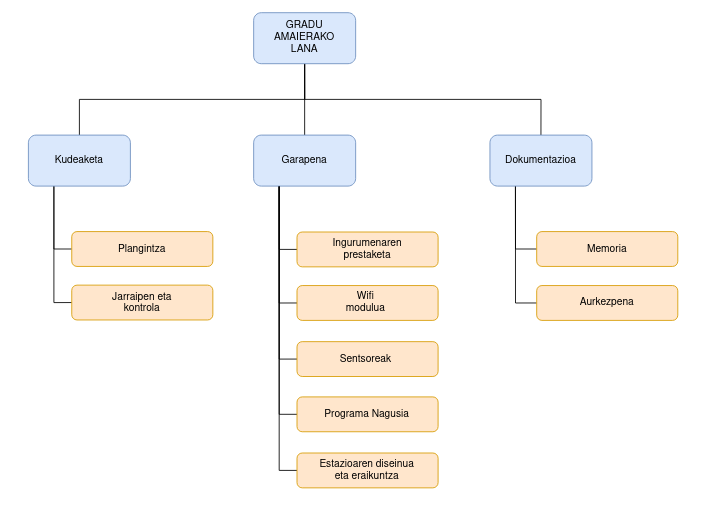
\includegraphics[width=.99\linewidth]{images/LDE3.png}
	\caption{\label{fig:lde} LDE diagrama}
\end{figure}

\paragraph{\textbf{Kudeaketa:}}
\begin{itemize}
    \item \textbf{Plangintza (P)} lan-paketeak, hasierako plangintza egiteko atazak eta behar badira, plangintza egunean mantentzeko behar daitezkeenak barne izango ditu.
    
        - \textbf{P.1:} Eskakizunen identifikazioa, hasierako erabakiak hartzea, informazioaren analisia eta zalantzen ebazpena. 
        
        - \textbf{P.2:} Hasierako plangintza, garapenerako ingurunea prestatzeko.
        
        - \textbf{P.3:} Plangintzaren eguneraketa, beharrezkoa bada.
    
    \item \textbf{Jarraipen eta kontrola (JK)} lan-paketeak proiektuaren garapen egokia bermatuko duten
atazak edukiko ditu eta konkretuki, proiektuko ataza bakoitzerako dedikazioen jarraipena eta epeen eta
espezifikazioen betetzea.

        - \textbf{JK.1:} Proiektuaren garapenari buruzko informazio garrantzitsua jaso.
        
        - \textbf{JK.2:} Planarekin, jarraipeneko informazioaren konparaketa, desbideratze esanguratsuen
eta sortzen diren arriskuen identifikazioa.
        
        - \textbf{JK.3:} Proiektuak arrakasta izan dezan, baldintzen bermatzea.
\end{itemize}
\paragraph{\textbf{Garapena:}}
\begin{itemize}
    \item \textbf{Ingurunearen prestaketa (IP)} lan paketean, proiektuan zehar estazioaren sorketa aurrera eramateko erabiliko diren baliabide guztien identifikazioa eta ikerkuntza sartzen dira.
        
        - \textbf{IP.1:} Beharrezkoa den softwarea identifikatu eta deskargatu.
        
        - \textbf{IP.2:} Baliabideen azterketa.
        
    \item \textbf{Wifi modulua (W)} lan-paketeak, \textbf{ESP-01} wifi moduluarekin zerikusia daukaten ataza guztiak edukiko ditu. %ikerketa, funtzionamendua, kodea 
    
        - \textbf{W.1:} Wifi moduluaren ikerketa.
        
        - \textbf{W.2:} Wifi modulua eta mikrokontrolagailua elkarlanean egoteko liburutegia sortu.
        
        - \textbf{W.3:} Sentsoreetatik jasotako datuak bidaltzeko protokolo baten diseinua.
        
    \item \textbf{Sentsoreak (S)} lan-paketeak, eguraldia aztertzeko balioko duten sentsoreen ikerketarekin zerikusia dauzkaten zereginak elkartuko ditu.
    
        - \textbf{S.1:} Erabili beharreko sentsoreen ikerketa.
        
        - \textbf{S.2:} Sentsoreak eskuratu edo eraiki.
        
        - \textbf{S.3:} Sentsoreak kontrolatzeko liburutegien kodeketa.
        
    %\item \textbf{Beharrezko Softwarea (SW)} lan-paketean proiektuan zehar, plakara kodea igotzeko edota kodea garatzeko erabiliko den sofwarearen azterketa dago barne.
    %\item \textbf{Liburutegiak sortu (L)} lan-paketeak ataza hauek bilduko ditu: Estazio meteorologikoa osatuko duten sentsore eta modulo bakoitza era egokian funtziona dezan kodetu beharreko programen garapena.
    
    \item \textbf{Programa Nagusia (PN)} lan paketean, programa nagusiaren garapena sartzen da.
    
        - \textbf{PN.1:} Wifi moduluaren programa, programa nagusiarekin integratu.
        
        - \textbf{PN.2:} Sentsoreen programak, programa nagusian integratu.
        
        - \textbf{PN.3:} Programa nagusiaren azken xehetasunak.
        
    \item \textbf{Estazioaren diseinua eta eraikuntza (E)} lan-paketea, estazioa diseinatzeko eta eraikitzeko atazek osatuko dute.
    
        - \textbf{E.1:} Estazioaren egitura diseinatu.
        
        - \textbf{E.2:} Eraikuntzarako beharrezkoak izango diren materialak eskuratu.
        
        - \textbf{E.3:} Proiektuko elektronika txukun jarri, gero behar den kaxatxoan sartzeko zirkuitua babestearren.
        
        - \textbf{E.4:} Estazioa eraiki.
        
\end{itemize}
\paragraph{\textbf{Dokumentazioa:}}
\begin{itemize}
    \item \textbf{Memoria (M)} lan-paketeak proiektuari buruzko memoria bat idaztea dauka helburu.
        
        - \textbf{M.1:} Memoriaren egitura prestatu.
        
        - \textbf{M.2:} Memoria osatu, proiektua nola garatu den eta plangintza azalduz.
        
    \item \textbf{Aurkezpena (A)} lan-paketearen barruan defentsa egunerako beharrezkoa izango den aurkezpena prestatzeko zereginak dauzka.
    
        - \textbf{A.1:} Aurkezpenaren garapena.
        
        - \textbf{A.2:} Aurkezpenaren prestaketa.
\end{itemize}

\newpage
\section{Denbora estimazioak}

%meter un poquico de txapuela y poner la tablica de las estimaciones de tiempos
Ondorengo irudiko taulan, aurreko ataleko LDE diagraman definitutako lan paketeen denbora estimazioak agertzen dira.

\begin{figure}[!htb]
	\centering
	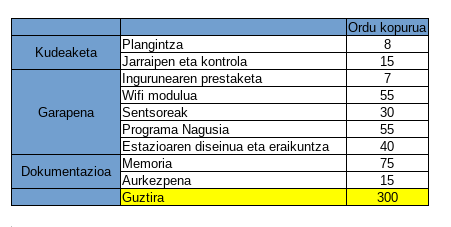
\includegraphics[width=.7\linewidth]{images/ordukop.png}
	\caption{\label{fig:lde} Lan paketeen ordu kopurua}
\end{figure}

Ikusten den bezala garrantzi handiena edukiko duten lan paketeak \textit{Garapena} eta \textit{Dokumentazioa} dira. Naiz eta \textit{Kudeaketan} ez diren hainbeste ordu eskainiko ezinbestekoak dira bertako atazak zuzen burutzea proiektuaren garapena espero den bezala joateko. Taulan ikusten den bezala guztira 300 ordu estimatu dira proiekturako, baina baliteke azkenean gehiago izatea. 


Hurrengo orrialdeko gantt diagramaren bidez, lan paketa hauen garapena denboran zehar ikus dezakegu. Era honetan errazagoa izango da ataza bakoitzaren hasiera eta bukaera datak egutegian finkatzea.

\newpage
\begin{figure}[!htb]
	\centering
	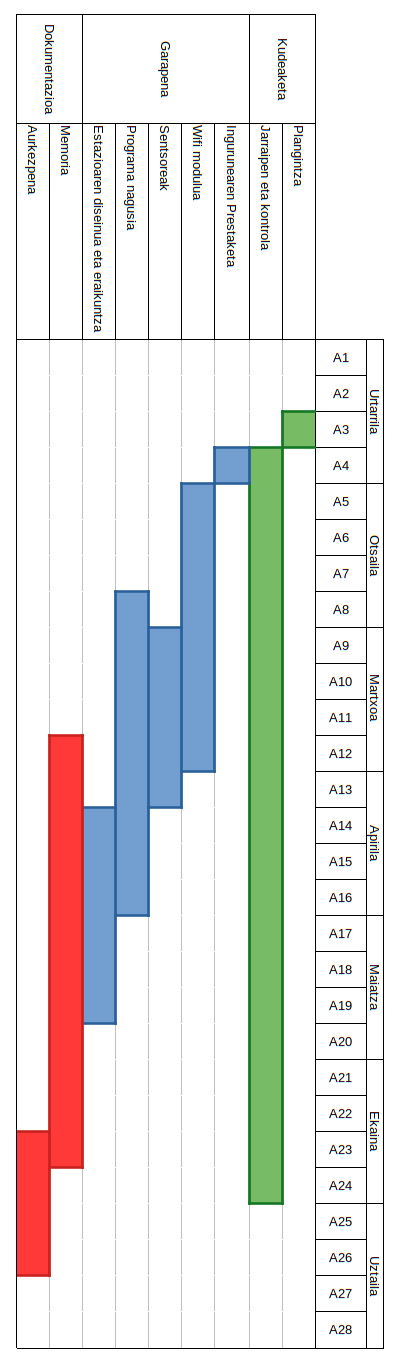
\includegraphics[width=.39\linewidth]{images/gantt2.png}
	\caption{\label{fig:lde} GANTT diagrama}
\end{figure}

\section{Kalitate plana}
Proiektuaren kalitate maila finkatzeko proiektuak bete beharko duen oinarrizko kalitate maila zehaztu behar da. Atal honetan proiektuak kalitate ona izan dezan, behar dituen ezaugarriak aipatuko dira.

\paragraph{\textbf{Oinarrizko betekizunak:}}
\begin{itemize}
    \item Wifi bidezko komunikazioa egon behar du estazioaren eta beste gailu baten artean.
    \item Sentsoreen funtzionamendua zuzena izan behar du.
    \item Proiektuko Hardware guztia babesteko egitura bat eraiki.
    \item Sentsoreek jasotako datuak beste gailu batetik kontsultatzeko ahalmena
    \item Kodea txukuna eta ulergarria izan behar du, interneten eskuragarri egongo baita edonorentzat.
\end{itemize}
\section{Arriskuak}

Proiektuaren garapena ondo joan dadin ezinbestekoa da egon daitezkeen arazoak identifikatzea, hauei soluzio bat bilatzeko. Arrisku guztiek ez dute eragin berdina izango proiektuarengan, eta hauek gertatzeko probabilitatea ez da berdina izango. Honako hauek dira proiektuan zehar gerta daitezkeen arazo batzuk.


\begin{itemize}
    \item \textbf{Hardwarearekin arazoak:} Mikrokontrolagailuetarako softwarea garatzerako orduan ohikoa da arazoak edukitzea, batzutan plakaren eta sistema eragilearen arteko komunikazioa ez dabil ondo edo sentsoreek emandako emaitzak ez dira esperotakoak. 
        
        - \textbf{Probabilitatea:} Altua
        
        - \textbf{Soluzioa:} Arazoari buruz informatu eta lehenbailehen zuzentzen ahalegindu. Erabilitako iturriak gordetzea komenigarria da berriro gertatu ezkero eskura izateko.
        
        
    \item \textbf{Datuen galera:} Proiektuan aurreratutako lan guztia galtzeko aukera badago. Hau gertatzeak, galdu den informazioaren arabera arazo handia izan liteke beraz ezinbestekoa da datuak ondo gordetzea. 
        
        - \textbf{Probabilitatea:} Ertaina.
        
        - \textbf{Soluzioa:} Informazio sistema ondo antolatua, eta segurtasun kopiak eduki. Komenigarria da \textit{Google Drive} bezalako plataforma batean datuak gordetzea orokorrean arazorik ematen ez duelako.
        
    \item \textbf{Covid-19:} Gaur egun bizitzen ari garen pandemia dela eta gaixotzeko aukera dago, proiektuaren garapena bertan behera utziz denboraldi batez.
        
        - \textbf{Probabilitatea:} Ertaina.
        
        - \textbf{Soluzioa:} Arduratsua izan eta behar diren neurriak hartu ez kutsatzeko.
        
    \item \textbf{Denbora falta:} Baliteke aurreko arazoen ondorioz edo planifikazio txarra egiteagatik proiektua bukatzeko denbora falta izatea, horrek entrega atzeratzera behartuko luke.
        
        - \textbf{Probabilitatea:} Txikia
        
        - \textbf{Soluzioa:} Planifikazioa kontu handiz egin ahalik eta xehetasun gehienak kontua hartuz.
    
\end{itemize}
    \chapter{Mikrokontroladorea}

\vspace{4cm}

Kapitulu honetan, proiektua aurrera eramateko erabili den mikrokontroladorea aztertuko da. Gailu honek dituen barne moduluak ezagutzera emango dira ere, hauen funtzionamendua azalduz eta estazioa behar den bezala funtzionatzeko konfiguratu behar diren erregistroak komentatuz.

\newpage

\section{Atmega328p mikrokontroladorea}

Proiektu honetarako erabili den kontrolagailua, \textbf{Atmega328p}-a izan da. Gailu hau, \textit{Atmel} konpainiak garatutako \textit{megaAVR} serieko potentzia baxuko 8 biteko CMOS mikrokontroladore bat da, AVR-rako hobetutako RISC arkitekturan oinarritutakoa. Mikrokontroladore hau oso ezaguna da, Arduino UNO txartelak erabiltzen baitu.

Arduino UNO plaka oso erabilia da elektronika proiektuen hasiberrian artean, bere merketasuna eta programatzeko erraztasunarengatik. Arduino plataforma handia bihurtu da 2003 urtean Arduino UNO-a atera zutenetik, eta gaur egun hamaika liburutegi eta plaka berri atera dituzte komunitatearen nahiak asetzeko, eta honek erraztasun handiak ematen ditu programatzerako orduan. Izan ere plataformak eskaintzen dituen baliabide hauke guztiak nahiko ilunak dira, programatzerako orduan funtzio sorta bat erabiltzen da eta ez dago argi erabilitako barne moduluen konfigurazioak nolakoak diren. Barne modulu hauen funtzionamendua eta konfigurazioak xehetasun guztiekin aztertu ahal izateko, proiektu honetan Atmega328p-a erregistro mailan programatuko da. 
%*zer da arduino y toda la txapa* *erregistro mailan y todo eso* *Poner las caracteristicas del arduino* y *poner el pinout*.  

\begin{figure}[htb]
	\centering
	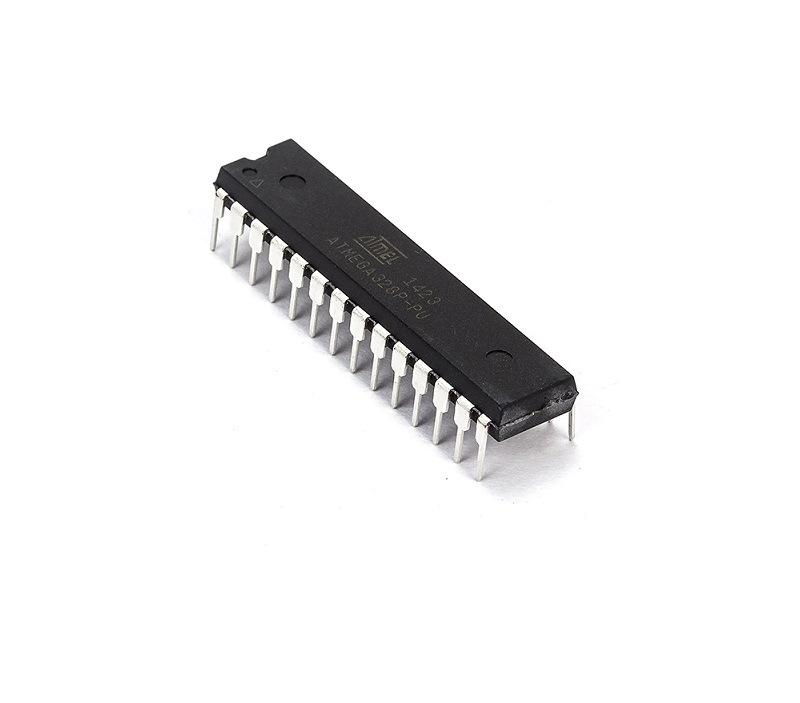
\includegraphics[width=.4\linewidth]{images/atmega.jpeg}
	\caption{\label{fig:bloke_diag} Atmega328p txipa}
\end{figure}

\section{Barne egitura}
Atal honetan, Atmega328p mikrokontroladoreak daukan barne egitura aztertuko dugu. Azpiko \ref{fig:bloke_diag} irudian ikusi daitezke ondoren ikertuko ditugun txiparen osagarri guztiak.

\begin{enumerate}
    \item \textbf{AVR prozesu unitatea:} Hau da mikrokontroladorearen zati garrantzitsuena, programen exekuzio zuzena bermatuko baitu. Prozesu unitateak \textit{Harvard} arkitektura erabiltzen du, programa eta datuentzako bus eta memoria desberdinak erabiliz. Aginduak erloju ziklo bakoitzean exekutatzen dira eta memoriak atzitzeko, kalkuluak egiteko, periferikoak kontrolatzeko eta etenak kudeatzeko gai da.
    \item \textbf{Timerrak:} Guztira 3 timer daude, non horietako bi 8 bitekoak diren eta bestea 16 bitekoa, guztiek prescaler berdina erabiltzen dute, baina konfigurazio desberdinekin. Horretaz gain 6 PWM kanal daude. %PWM kanalak
    \item \textbf{Komunikazio interfazeak:} Hiru desberdin dauzka txip honek, USART, SPI eta TWI. Interfaze hauetako bakoitzak datuak jaso eta bidali ahal izateko aurredefinitutako eta komunikaziorako prest dauden sarrera/irteera pinak erabiltzen dituzte.
    \item \textbf{Memoriak:} Hiru dira Atmega328p-ak dituen memoriak, 32k byteko Programa Flash memoria programak gordetzeko, 2k byteko SRAM memoria bat, programak sortzen dituen aldagaiak gorde ahal izateko eta azkenik 1k byteko EEPROM memoria bat informazio iraungarria gorde ahal izateko.
    \item \textbf{ADC modulua:} seinale analogiko bat, 10 biteko datu batean bihurtzeko gai da (0-tik 1023-ra). Modulu honek 6 sarrera/irteera pin ditu. %analog comparer
\end{enumerate}
\newpage
\begin{figure}[htb]
	\centering
	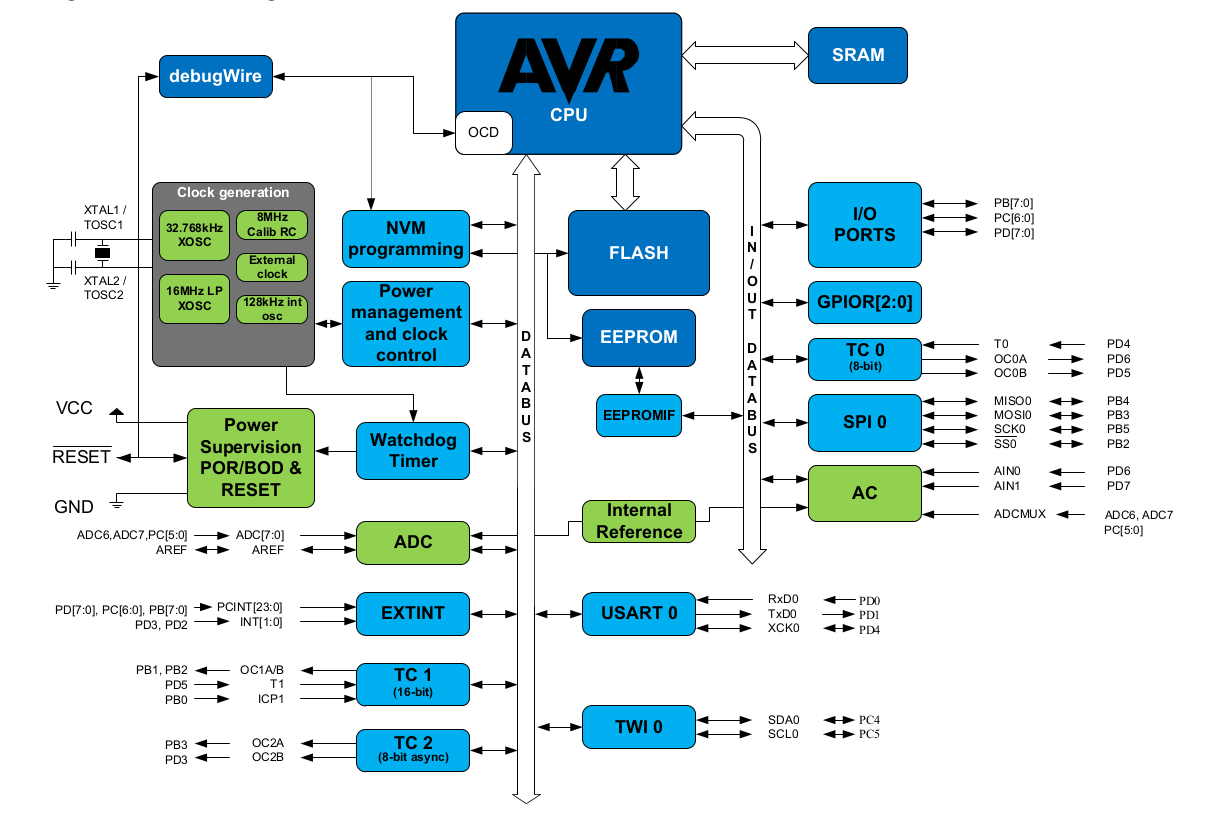
\includegraphics[width=.99\linewidth]{images/bloke_diagrama.png}
	\caption{\label{fig:bloke_diag} Atmega328p txiparen bloke diagrama}
\end{figure}


\section{Sarrera/Irteera hankatxoak}

Atal honetan Atmega328p txipak dituen hankatxoak aztertuko ditugu, guztira 28 dira eta hauetako bakoitza hainbat gauzetarako erabili daitezke. Hona hemen \ref{fig:pinout} irudian agertzen diren hankatxoen azalpena.

\begin{enumerate}
    \item \textbf{VCC: }
    \item \textbf{GND:}
    \item \textbf{PORTB:}
    \item \textbf{PORTC:}
    \item \textbf{PC6/$\overline{RESET}$:}
    \item \textbf{PORTD:}
    \item \textbf{AV$_{CC}$:}
    \item \textbf{AREF:}
    \item \textbf{ADC:}
\end{enumerate}

% azaldu hankatxoak taldeka PCINT, etenak, analog, digitak tx, rx, SDA, SCL, TWI....
\newpage
\begin{figure}[htb]
	\centering
	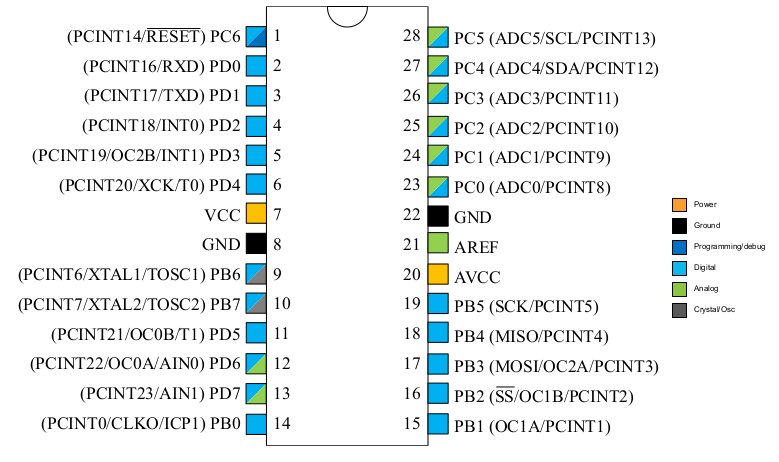
\includegraphics[width=.8\linewidth]{images/pinak.png}
	\caption{\label{fig:pinout} Atmega328p txiparen hankatxoen diagrama}
\end{figure}
    \chapter{Erabilitako sentsore eta moduluak}

\vspace{4cm}

Kapitulu honetan, erabili diren moduluak azalduko dira.....

\newpage

\section{ESP8266 wifi modulua}
\section{DHT11 tenperatura eta hezetasun sentsorea}
    
    
    \bibliographystyle{IEEEtranS}  
    \bibliography{references.bib}

\end{document}

